\documentclass[10pt]{beamer}



\mode<presentation>
{
  \usetheme{Berkeley}
%	\usetheme{Berlin}
%   \usecolortheme{}
%   \useinnertheme{circles}
   
  \setbeamercovered{transparent}

}


\usepackage[english]{babel}
\usepackage[utf8]{inputenc}
\usepackage{times}
\usepackage[T1]{fontenc}
\usepackage{multimedia}
\usepackage[absolute,overlay]{textpos}
\usepackage{graphicx}

\usepackage{xcolor}
\usepackage{amsmath}
\usepackage[absolute,overlay]{textpos}
\usepackage{physics}

\graphicspath{{./media/images/}}

\definecolor{paint}{RGB}{150,0,0}
\setbeamercolor {structure} {fg=paint}
\setbeamercolor{title}{fg=black}
\setbeamertemplate{itemize items}[circle]

\newcommand{\jsqrt}[2]{\bqty{ #1 #1 | #2 #2 }}
\newcommand{\ksqrt}[2]{\bqty{ #1 #2 | #2 #1 }}
\newcommand\mf[1]{\mathbf{#1}}
\newcommand\dens{\rho(\mathbf{r})}
\newcommand\densin{\rho^{in}(\mathbf{r})}
\newcommand\densout{\rho^{out}(\mathbf{r})}
\newcommand\rdens{\tilde{\rho}(\mathbf{G})}
\newcommand\erre{\mathbf{r}}
\newcommand\GI{\mathbf{G}}
\newcommand\QE{\textsc{Quantum} ESPRESSO }
\newcommand\numbands{n_{bands}}
\newcommand\numG{n_{G}}
\newcommand\numR{n_{R}}
\newcommand\bigO{\mathcal{O}}
\newcommand\CO{Co\textsubscript{3}O\textsubscript{4} } 


\title[Tuning the computational architecture for Quantum Espresso ab initio calculation of nanostructures] % (optional, use only with long paper titles)
{Tuning the computational architecture for Quantum Espresso ab initio calculation of nanostructures}

\author[Giorgio Ruffa] 
{Giorgio Ruffa}
\institute[Università degli Studi di Milano]{Università degli Studi di Milano}

\date{28 Aprile 2016} 

\subject{}


\begin{document}

% ********** 1 slide *****************
\begin{frame}
  \titlepage
\end{frame}

\section{Introduzione}

% ********** 2 slide *****************
\begin{frame}{Introduzione}

\begin{textblock*}{3cm}(2cm,2cm) 
	
\includegraphics[width=3cm]{beam_qe_logo.jpg}
\end{textblock*}

\begin{textblock*}{3cm}(9cm,2cm)
	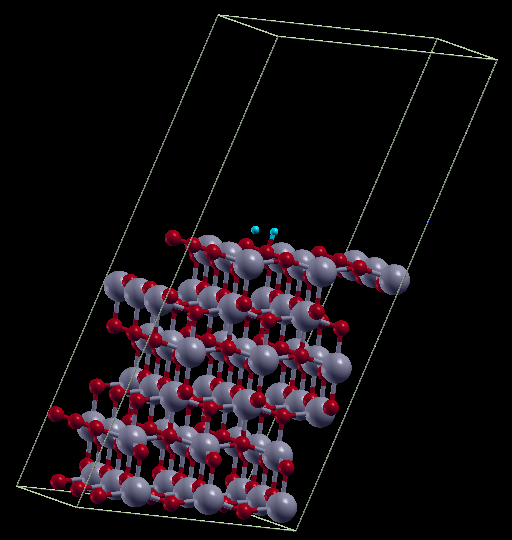
\includegraphics[width=3cm]{titania_crystal.png}
\end{textblock*}

\begin{textblock*}{10cm}(2cm,4.5cm)
Density Functional Theory (DFT) \\
Equazioni Kohn-Sham : 
\begin{align*}
&\lbrace  - \frac{1}{2} \nabla_{i}^2+ v_{eff}(\erre) \rbrace 	\psi_{i}^{KS}(\erre) = \varepsilon_{i}^{KS} \psi_{i}^{KS}(\erre)\\
&v_{eff}(\erre) = v_{ion}(\erre) + v_{h}(\erre) + v_{xc}(\erre) \\ 
&v_{h}(\erre) = \int \frac{\rho(\erre')}{\mid \erre - \erre'\mid} \dd{\erre'}\\ 
&v_{xc}(\erre) =	\frac{\var{E_{xc}[\dens]}}{\var{\dens}}
\end{align*}

\end{textblock*}


\end{frame}



\end{document}